%% LyX 2.3.2-2 created this file.  For more info, see http://www.lyx.org/.
%% Do not edit unless you really know what you are doing.
\documentclass[english]{upeeei}
\usepackage[latin9]{inputenc}
\setcounter{secnumdepth}{3}
\setcounter{tocdepth}{3}
\usepackage[active]{srcltx}
\usepackage{float}
\usepackage{units}
\usepackage{graphicx}
\usepackage[hyphens]{url}
\usepackage{hyperref}
\hypersetup{breaklinks=true}
%\usepackage[table,xcdraw]{xcolor}
\usepackage{url}
\makeatletter

%%%%%%%%%%%%%%%%%%%%%%%%%%%%%% LyX specific LaTeX commands.
\providecommand{\LyX}{L\kern-.1667em\lower.25em\hbox{Y}\kern-.125emX\@}
%% Because html converters don't know tabularnewline
\providecommand{\tabularnewline}{\\}

\@ifundefined{showcaptionsetup}{}{%
 \PassOptionsToPackage{caption=false}{subfig}}
\usepackage{subfig}
\makeatother

\usepackage{babel}
\begin{document}
%%% UP EEEI undergraduate project template
%% v0.1 by Louis P. Alarcon 11/22/2011
%%
%% LyX template - use with the following files:
%% 	uct10_new.clo, uct11_new.clo, uct12_new.clo, upeeei.cls, upeeei.layout
%%
%% Place project title here
\title{Implementing a Hybrid Solar-Grid System and Load Profile Dataset Creation in the Philippines} 

%%
%% Author information

\author{
%% Louis Poblete Alarc\'on\\ xxxx-xxxxx\\ \emph{Ph.D. Electrical Engineering and Computer Sciences} \and
Pamela Jane Aquino Maucesa\\ 2014-10134\\ \emph{BS Computer Engineering}
\and
Raphael Cyron Marcelo Robles\\ 2015-06938\\ \emph{BS Computer Engineering}
\and
Mary Angelson Coronel\\ 2014-64398\\ \emph{BS Electronics and Communications Engineering}
\and
Jonas Eumenda Ermeo\\ 2013-39597\\ \emph{BS Electronics and Communications Engineering}
\and
}

%%
%% Month and year of submission/graduation
\degreeyear{2019} 
\degreesemester{December} 

% Put your advisers here:
\chair{Wilbert Jethro Ramirez Limjoco, M.S.} 
\othermembers{Lew Andrew Ravelas Tria, Ph.D.} 
\numberofmembers{2} 

\field{Electrical/Computer/Electronics and Communications Engineering} 
\campus{Diliman} 

\maketitle 
% \approvalpage 
% \copyrightpage 
\begin{abstract} 

%Your abstract goes here...
%Energy source is now considered one of the basic needs of a human since it was used everywhere but its regeneration cannot catch up to its usage.  

Energy resources are being used by humans in most day to day activities. However, these resources are not managed efficiently, like in the Philippines, causing energy scarcity in some areas.  Because of this, there is a need to create a system that is capable of managing these resources to accommodate the needs of the people.  This study aims to create an energy management system that can efficiently distribute and manage available energy sources coming from solar power or electric grid depending on the load profiles of the appliances. In order to create this kind of system, there is a need to consider the behavior of appliances being used in the country. However, there are currently no available load profile datasets of appliances in the country thus the need to create one.

%With this, it also needs a reliable dataset that can describe the behavior of appliances being used in the country but in the present, there are no existing one in the country so there is a need to create one.

\abstractsignature\end{abstract}

\begin{frontmatter} 

\setlength{\parskip}{0pt}

\tableofcontents{}

\listoffigures

\listoftables

\end{frontmatter} 

\def\MASTERDOC{true}

\cleardoublepage{}

\chapter{Introduction\label{cha:Introduction}}

%This section ideally contains the following sub-sections: background of the project, project objectives, and overview of the project.

\section{Background of the Project}

Access to energy does a lot of things to all people ranging from connecting with each other through our gadgets to providing a livelihood for our families. Despite this, nearly 1.3 billion people or one out of five people on Earth do not have access to electricity  \cite{Politico.2015}. Energy is not an unlimited resource and that is why energy conservation and alternative sources have been greatly researched. For a more bounded and specific setting, we take the Philippines as our main example. 

In the Philippines, Luzon is at a 94.8\% electrification level which means that the island group is now in need of savings for energy consumption \cite{solar-manila}. Energy scarcity is a problem not just in the geographically hard to reach areas but also in the urban areas. In Luzon alone, there is a continuing Yellow and Red alerts being experienced that may eventually lead to a serious power supply shortage in the next few years \cite{Inquirer.2019}. Republic Act No. 11285 addresses these energy problems and institutionalized energy efficiency and conservation \cite{RA11825}. 

In addition, some rural areas in the Philippines do not have access to reliable and constant electricity. Harnessing solar energy has presented itself as a possible solution to reduce dependence on non-renewable sources of energy. However, solar energy can be very variable and implementing a purely solar dependent source would  impractical. Thus, there is a need to create a hybrid solar-grid system that can properly manage the electrical energy we have through monitoring and forecasting of the load and incoming power from the photovoltaic panels.

To develop this kind of system, there is a need for datasets to examine the load profiles of the appliances and to know hot to manage electrical energy efficiently. There are a lot of datasets available that can be used in the field of non-intrusive load monitoring  (NILM). However, there is a lack of research on creating the dataset of the load profiles of appliances in the Philippines, and the publicly available datasets may not be applicable for the NILM researches in the country. It is possible that the electrical characteristics and the devices being used in a household can vary from different countries, especially since the Philippines have different conditions (climate, seasons, temperature) in comparison to other countries that has an effect on the behavior of appliances being used as well as the consumers. Hence, there is need for an energy reference dataset based in the Philippines to help create a reliable and efficient energy monitoring and management system in the country.  This study aims to create a dataset for load profiles of appliances applicable for Philippine setting and to have a system that can optimally manage energy sources available.

\section{Documentation Flow and Organization}

For the flow of the rest of the paper, Chapter \ref{cha:RRW} will look at different energy sources, energy utilization, and load forecasting techniques.  This chapter will focus on publicly available works that may be used as basis for this study. Chapter \ref{cha:ProbStatement} will discuss the use and importance of the study as well as the objectives of the study. The proponents will also discuss the scope and limitations of the study in this chapter. Lastly, Chapter \ref{cha:Methodology} will contain the framework and methodology that will be followed by the proponents in conducting the study.

\cleardoublepage{}

\chapter{Related Work\label{cha:RRW}}

%A review of previous work and other materials related to the project shall be written here. Make sure you do proper citations of original materials taken from various sources. For example, if this sentence is taken from reference \#1 in my bibliography, it should be referenced just like this {[}1{]}. Avoid copying sources word for word. Always paraphrase. \textquotedblleft If it cannot be avoided, enclose the cited material in double quotes just like this\textquotedblright{} {[}2{]}. If this whole paragraph was taken from two different sources, then the citations may be written this way {[}3{]}, {[}4{]}. 

% %%Highlight flow
Electrical load forecasting is an important process in efficient utilization and management of electrical energy resources. This chapter will first tackle the nature of the energy sources that will be managed, mainly focusing on solar energy. Second, the energy utilization of appliances will be discussed including the existing datasets being used for researches. Finally, the existing load forecasting techniques where such datasets are analyzed and synthesized will be discussed.

%This chapter will first tackle different kinds of energy sources, mainly focusing on solar energy, second, energy utilization, and then finally, existing load forecasting techniques being used.

% %%critique

\section{Energy Sources}
There are different kinds of energy sources existing nowadays like power plants.  The paper will only focus on the type which will be used in research, solar energy.

Researches on providing renewable energy sources is emerging since it is already existing in nature whether people use it or not which makes it economically profitable.  It also does not harm the environment \cite{renew-energy}.  One example of these kinds of energy sources is solar energy.

Solar energy is the kind of energy source that generates electricity from sunlight.  This kind of energy source is growing because of its efficiency compared to others.  There are two ways to implement solar energy.  One can use photovoltaic (PV) systems where energy is generated through photovoltaic effect, or Concentrated Solar Power(CSP) where energy is generated through heating fluids by mirrors and concentrators \cite{solar-power}.  %It is necessary to monitor incoming power to the system especially with the highly variable power output of a photovoltaic (PV) system due to its dependency on solar irradiance and other meteorological factors \cite{HOSSAIN2017395}.

Since the nature of energy from renewable resources like solar energy can be highly variable, the use of batteries are required to even out the power distributions \cite{soc-battery}. This shows the need to monitor the state of the battery in order to properly manage the system. It can also result for a longer lifetime of the battery \cite{soc-soh}. One common example that uses battery as its energy source are electric vehicles.  It uses rechargeable battery for propulsion and in turn, no emission occurs compared to other vehicles \cite{soc-soh}. Studies have shown to use the ampere-hour counting method or the coulomb counting method in calculating the current state of charge (SOC) \cite{soc-battery},\cite{soc-soh}. The SoC provides the percentage (\%) of battery capacity, or its level of charge relative to its capacity, which is needed in order to manage the energy system. Other methods for measuring the SoC of the battery like using the Thevenin model also proved to be reliable, however can also be difficult to model and determine its parameters \cite{soc-predict}. The coulomb counting method can provide accurate values for the SoC and is generally applicable for SoC estimation of any battery based on measurements. The method seems to be accurate and general enough to be applicable for SoC estimation needed in the project.

\section{Energy Utilization}

Since non-renewable energy sources is still cheaper compared to renewable energy sources (e.g. solar power) and renewable ones are not regenerating easily, energy utilization is a must to efficiently use these.  Energy utilization means efficiently managing and utilizing energy sources being used \cite{energy-util}.  Energy utilization is not just limiting the use of the people of the energy sources.  The first step in doing so is knowing the demand of it and how people frequently use it \cite{load-profile-analysis}.  This can be done through the analysis of datasets about the load profiles of the appliances since it provides details about the power consumption of each appliances being used.  For the past researches, datasets where used for the forecasting of power consumption of either households or institutional blocks.  There are many available datasets of load profiles of appliances from different countries.  Some of these are REDD \cite{REDD}, datasets from openei.org, and many more.
%% pican / sir yap
%% openei 
%% redd

One example of dataset is called Reference Energy Disaggregation Dataset (REDD).  REDD is a freely available dataset containing power consumption of several households.  The creation of this dataset aims to help researches on energy disaggregation. \cite{REDD}

In creating the dataset, several households in Boston and San Francisco, both cities in the United States, were involved for the data collection for a few months.  The researchers recorded the whole home electricity signal up to 24 individual circuits, up to 20 plug-level monitors in each home. Figure \ref{fig:redd-data} shows an example energy consumption data over a day in a single household.

\begin{figure}[H]
\begin{centering}
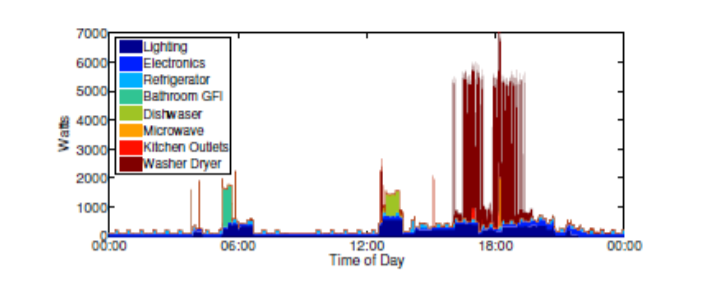
\includegraphics[width=0.8\columnwidth]{images/redd-data.png}
\par\end{centering}
\caption{\protect An example of energy consumption data over a day in one household \cite{REDD} \label{fig:redd-data}}
\end{figure}

Another dataset describing the hourly load profiles for sixteen (16) commercial and residential buildings in the United States.  It considered different kinds of appliances used in a commercial and residential buildings \cite{tmy3}.  Building characteristics is shown in Table \ref{tab:tmy3-table}.

\begin{table}[H]
\caption{Base Load Model (Building America B10 Benchmark) \label{tab:tmy3-table}}

\centering{}%
\resizebox{\textwidth}{!}{%
\begin{tabular}{cccccc}
\cline{2-6}
\multicolumn{1}{c|}{} & \multicolumn{5}{c|}{\textbf{Selected Building Fuel Types}} \\ \cline{2-6} 
\multicolumn{1}{c|}{\textbf{}} & \multicolumn{1}{c|}{\textbf{Very Cold/Cold}} & \multicolumn{1}{c|}{\textbf{Mixed-Humid}} & \multicolumn{1}{c|}{\textbf{Mixed-Dry/Hot-Dry}} & \multicolumn{1}{c|}{\textbf{Hot-Humid}} & \multicolumn{1}{c|}{\textbf{Marine}} \\ \hline
\multicolumn{1}{|c|}{\textbf{Space Heating}} & \multicolumn{1}{c|}{Natural Gas} & \multicolumn{1}{c|}{Natural Gas} & \multicolumn{1}{c|}{Natural Gas} & \multicolumn{1}{c|}{Natural Gas} & \multicolumn{1}{c|}{Natural Gas} \\ \hline
\multicolumn{1}{|c|}{\textbf{Air Conditioning}} & \multicolumn{1}{c|}{Yes} & \multicolumn{1}{c|}{Yes} & \multicolumn{1}{c|}{Yes} & \multicolumn{1}{c|}{Yes} & \multicolumn{1}{c|}{No} \\ \hline
\multicolumn{1}{|c|}{\textbf{Water Heating}} & \multicolumn{1}{c|}{Natural Gas} & \multicolumn{1}{c|}{Electric} & \multicolumn{1}{c|}{Natural Gas} & \multicolumn{1}{c|}{Electric} & \multicolumn{1}{c|}{Natural Gas} \\ \hline
 &  &  &  &  &  \\ \cline{2-6} 
\multicolumn{1}{c|}{\textbf{}} & \multicolumn{5}{c|}{\textbf{Selected Building Structure Types}} \\ \cline{2-6} 
\multicolumn{1}{c|}{\textbf{}} & \multicolumn{1}{c|}{\textbf{Very Cold/Cold}} & \multicolumn{1}{c|}{\textbf{Mixed-Humid}} & \multicolumn{1}{c|}{\textbf{Mixed-Dry/Hot-Dry}} & \multicolumn{1}{c|}{\textbf{Hot-Humid}} & \multicolumn{1}{c|}{\textbf{Marine}} \\ \hline
\multicolumn{1}{|c|}{\textbf{Total Size (sq. ft.)}} & \multicolumn{1}{c|}{2696} & \multicolumn{1}{c|}{2546} & \multicolumn{1}{c|}{2000} & \multicolumn{1}{c|}{2023} & \multicolumn{1}{c|}{2090} \\ \hline
\multicolumn{1}{|c|}{\textbf{Urban and Rural}} & \multicolumn{1}{c|}{Urban} & \multicolumn{1}{c|}{Urban} & \multicolumn{1}{c|}{Urban} & \multicolumn{1}{c|}{Urban} & \multicolumn{1}{c|}{Urban} \\ \hline
\multicolumn{1}{|c|}{\textbf{Metropolitan and Micropolitan}} & \multicolumn{1}{c|}{Metro} & \multicolumn{1}{c|}{Metro} & \multicolumn{1}{c|}{Metro} & \multicolumn{1}{c|}{Metro} & \multicolumn{1}{c|}{Metro} \\ \hline
\multicolumn{1}{|c|}{\textbf{Number of Stories/Levels}} & \multicolumn{1}{c|}{1 Story} & \multicolumn{1}{c|}{1 Story} & \multicolumn{1}{c|}{1 Story} & \multicolumn{1}{c|}{1 Story} & \multicolumn{1}{c|}{1 Story} \\ \hline
\multicolumn{1}{|c|}{\textbf{Major Outside Wall Construction}} & \multicolumn{1}{c|}{Siding (Aluminum, Vinyl, Steel)} & \multicolumn{1}{c|}{Siding (Aluminum, Vinyl, Steel)} & \multicolumn{1}{c|}{Stucco} & \multicolumn{1}{c|}{Brick} & \multicolumn{1}{c|}{Wood} \\ \hline
\multicolumn{1}{|c|}{\textbf{Major Roofing Material}} & \multicolumn{1}{c|}{Ceramic or Clay Tiles} & \multicolumn{1}{c|}{Ceramic or Clay Tiles} & \multicolumn{1}{c|}{Ceramic or Clay Tiles} & \multicolumn{1}{c|}{Ceramic or Clay Tiles} & \multicolumn{1}{c|}{Ceramic or Clay Tiles} \\ \hline
\multicolumn{1}{|c|}{\textbf{Foundation/Basement of Single-Family}} & \multicolumn{1}{c|}{Basement} & \multicolumn{1}{c|}{Concrete Slab} & \multicolumn{1}{c|}{Concrete Slab} & \multicolumn{1}{c|}{Concrete Slab} & \multicolumn{1}{c|}{Crawlspace} \\ \hline
\multicolumn{1}{|c|}{\textbf{Bedrooms}} & \multicolumn{1}{c|}{3} & \multicolumn{1}{c|}{3} & \multicolumn{1}{c|}{3} & \multicolumn{1}{c|}{3} & \multicolumn{1}{c|}{3} \\ \hline
\multicolumn{1}{|c|}{\textbf{Full Bathrooms}} & \multicolumn{1}{c|}{1} & \multicolumn{1}{c|}{1} & \multicolumn{1}{c|}{2} & \multicolumn{1}{c|}{2} & \multicolumn{1}{c|}{1} \\ \hline
\multicolumn{1}{|c|}{\textbf{Half Bathrooms}} & \multicolumn{1}{c|}{None} & \multicolumn{1}{c|}{None} & \multicolumn{1}{c|}{None} & \multicolumn{1}{c|}{None} & \multicolumn{1}{c|}{None} \\ \hline
\multicolumn{1}{|c|}{\textbf{Basement Single-Family Homes}} & \multicolumn{1}{c|}{Yes} & \multicolumn{1}{c|}{No} & \multicolumn{1}{c|}{No} & \multicolumn{1}{c|}{No} & \multicolumn{1}{c|}{No} \\ \hline
\multicolumn{1}{|c|}{\textbf{Finished Basement}} & \multicolumn{1}{c|}{No} & \multicolumn{1}{c|}{No Basement} & \multicolumn{1}{c|}{No Basement} & \multicolumn{1}{c|}{No Basement} & \multicolumn{1}{c|}{No Basement} \\ \hline
\multicolumn{1}{|c|}{\textbf{Type of Glass in Windows}} & \multicolumn{1}{c|}{Double-pane Glass} & \multicolumn{1}{c|}{Double-pane Glass} & \multicolumn{1}{c|}{Single-pane Glass} & \multicolumn{1}{c|}{Single-pane Glass} & \multicolumn{1}{c|}{Double-pane Glass} \\ \hline
\multicolumn{1}{l}{} & \multicolumn{1}{l}{} & \multicolumn{1}{l}{} & \multicolumn{1}{l}{} & \multicolumn{1}{l}{} & \multicolumn{1}{l}{} \\ \cline{2-6} 
\multicolumn{1}{l|}{} & \multicolumn{5}{c|}{\textbf{Selected Building Design Type}} \\ \cline{2-6} 
\multicolumn{1}{l|}{} & \multicolumn{5}{c|}{\textbf{ALL OTHER OPTIONS SET TO B10 BENCHMARK HOUSE}} \\ \cline{2-6} 
\end{tabular}%
}
\end{table}

On the other hand, load profiling was also done in Cankiri, Turkey where the power consumption of basic home 12 different appliances used in the region are taken one-second intervals \cite{Determine}. The following devices are used by households with only two occupants from October to December 2016. The table below shows the plug ID number of the device used in the study, brand, model, efficiency class, and amount of power consumption of all the devices used by the residents in the span of three months.

\begin{figure}[H]
\begin{centering}
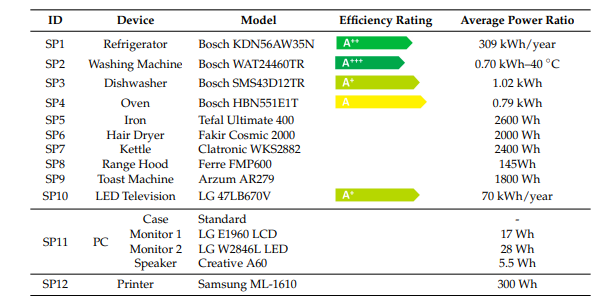
\includegraphics[width=0.8\columnwidth]{images/1.png}
\par\end{centering}
\caption{\protect Devices used in 12 households in Cankiri, Turkey for load profiling\cite{Determine} \label{fig:cankiri}}
\end{figure}

In order to obtain the power consumption of each device with high resolution, the researchers designed a system which consists of Radxa RockPro single board computer and an Edimaz Smart Plug wireless power meter. Data of the power consumption of the devices were taken by connecting the Edimax Smart Plug, while the Radxa RockPro SBC minicomputer with Quad Core ARM processor monitored the wireless power measurement plug as it took the consumed power value of each device. Data from the smart plugs were collected using a software based on Java and a Linux operating system \cite{Determine}.

\begin{figure}[H]
\begin{centering}
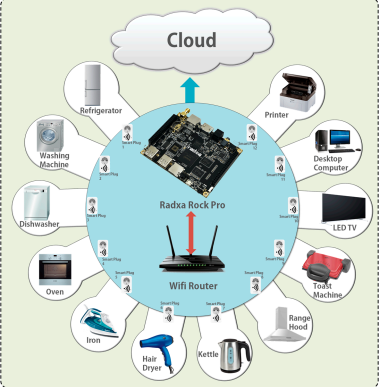
\includegraphics[width=0.8\columnwidth]{images/3.png}
\par\end{centering}
\caption{\protect System block diagram \cite{Determine} \label{fig:sysblockdiag}}
\end{figure}

The figure below shows the data for November 2016. There are similar devices used in the Philippines that are also used in this study except that the average household size here in the country is around 4 or 5 people \cite{PSA} whereas the study only based on a 2-person household. It is also worth noting that on the month of November, the average temperature in Cankiri, Turkey is at $6.5\ ^{o}$C \cite{cc} , while average temperature in Metro Manila ranges from $24\ ^{o}$C to $33\ ^{o}$C \cite{accu}. While both the Philippines and Turkey generally runs on 220 Volts, the former operates on 60 Hertz, while the later operates on 50 Hertz  \cite{socket}. Due to these differences, the load profile obtained by this study cannot be applied in the Philippine setting, and thus the need to create a data set which is acclimatized for the country.

\begin{figure}[H]
\begin{centering}
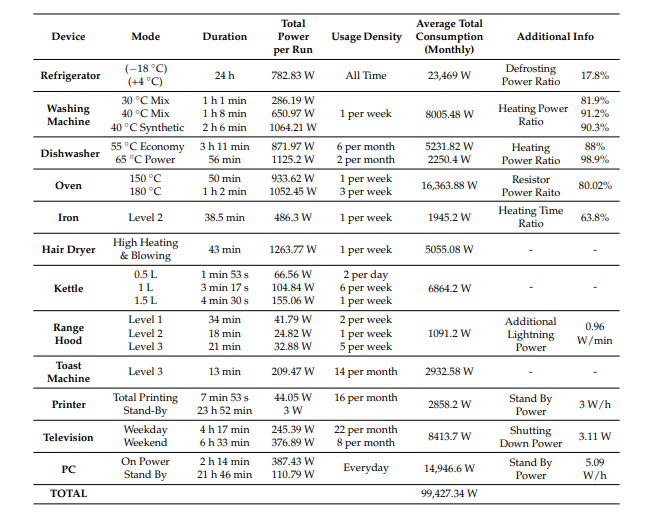
\includegraphics[width=0.8\columnwidth]{images/2.png}
\par\end{centering}
\caption{\protect Average power consumption of devices for the 12 households in Cankiri, Turkey for November 2016 \cite{Determine} \label{fig:turkey}}
 \end{figure}

Another study was conducted in the University of the Philippines - Diliman, specifically in the Ubiquitous Computing Laboratory, wherein it implemented an home automation system called Smart Domotix \cite{Domotix}.  Figure \ref{fig:domotix} shows its system overview. The components of the system are the following:

\begin{itemize}
    \item a smart plug connected to the appliances to be able to control and monitor its usage
    \item a main controller that serves as a gateway to the internet
    \item a server for storing information about the appliances
\end{itemize}

\begin{figure}[H]
\begin{centering}
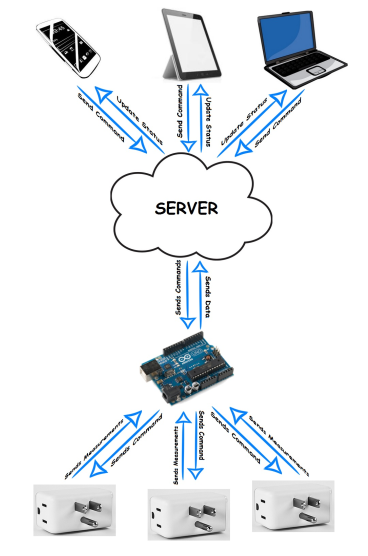
\includegraphics[width=0.5\columnwidth]{images/domotix-sys.png}
\par\end{centering}
\caption{\protect Smart Domotix System Overview \cite{Domotix} \label{fig:domotix}}
\end{figure}

For the smart plug, it is the one responsible for interacting with the appliances since it is the one that has the control to turn it ON or OFF, and to be able to monitor its power consumption.  The architecture of the smart plug is shown in Figure \ref{fig:smart-plug}.

\begin{figure}[H]
\begin{centering}
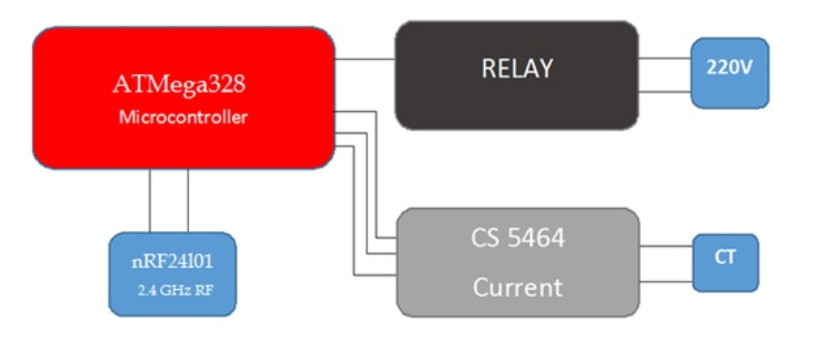
\includegraphics[width=0.6\columnwidth]{images/domotix-plug.png}
\par\end{centering}
\caption{\protect Smart Plug Architecture \cite{Domotix} \label{fig:smart-plug}}
\end{figure}

ATMega328 microcontroller serves as processor of the smart plug since it is the one that handles the commands sent by the main controller.  They used radio frequency as the medium at 2.4 GHz to communicate to the main controller wirelessly through the RF module nRF24101.  For power monitoring feature of the system, they used CS5464 chip to convert the current detected by current transformer (CT) (Figure \ref{fig:domotix-ct}) into a 32-bit digital representation.  Calibration and mapping to the real power value was done because the data readings in the chip are not yet the real one.  Through the calibration curve, the ATMega328 was able to convert the data readings to its real power and send it to the main controller every second.

\begin{figure}[H]
\begin{centering}
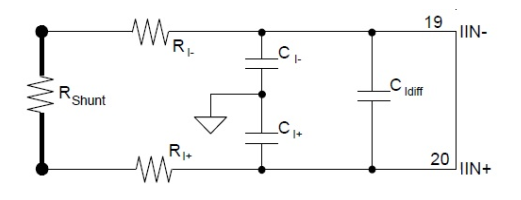
\includegraphics[width=0.5\columnwidth]{images/domotix-ct.png}
\par\end{centering}
\caption{\protect Current Transformer Circuit \cite{Domotix} \label{fig:domotix-ct}}
\end{figure}

For the user side, for them to be able to control the appliances, they created a mobile and web application with the following features:

\begin{itemize}
    \item turn ON or OFF a specific appliance
    \item schedule the usage of the specific appliances (e.g. Air conditioner set to run at 7:00 pm)
    \item view the power consumption of each appliance per day, week, month, and year
\end{itemize}

\begin{figure}[H]
    \centering
  \subfloat[Mobile App\label{fig:Domotix-mobile}]{%
       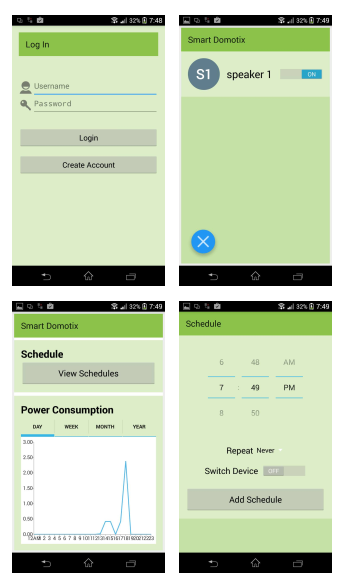
\includegraphics[width=0.4\linewidth]{images/domotix-mobile.png}}
  \subfloat[Web App\label{fig:Domotix-web}]{%
        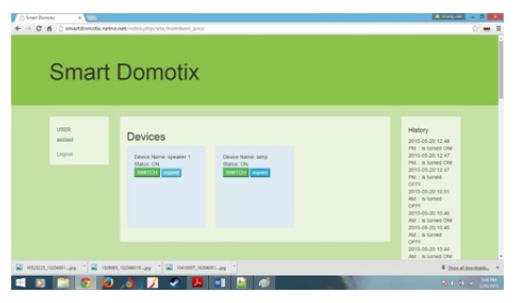
\includegraphics[width=0.4\linewidth]{images/domotix-web.png}}
  \caption{ (a) Mobile Application (b) Web Application User Interface of Smart Domotix \cite{Domotix}} \label{fig:Domotix}
\end{figure}

The system were able to achieve an average percent error of 2.27\% for monitoring the power consumption of each appliances and at the same time, the mobile and web application created was user friendly, plug and play based from the survey they conducted.

\section{Energy Forecasting Techniques}
%Bridge Energy Util and Energy Forecasting Techniques
Aside from the analysis of the load profiles of the appliances being used, forecasting the incoming power and load demand from the system is also important in efficiently managing energy sources. Different existing methods being used to forecast the energy from the PV systems, the state of charge of the battery and demand of energy will be discussed in this section.

\subsection{PV Power Forecasting}
Studies have shown to use various forecasting models such as persistent model, auto-regressive integrated moving average (ARIMA), k-nearest-neighbors (kNNs), and artificial neural networks (ANNs) to predict 1 and 2 hour-ahead average power outputs and has shown results of better performance of ANN-based forecasting models compared to other forecasting techniques and that it can be further improved with a genetic algorithm optimization of the ANN parameters \cite{PEDRO20122017}. More recent studies from the University of Malaya has shown the use of extreme learning machine (ELM) for forecasting short term output power of PV systems. Extreme machine learning selects hidden nodes randomly to determine the output weights of single-hidden layer feedforward neural networks and have proven to be faster than conventional popular learning algorithms \cite{HUANG2006489}. The system uses an irradiance, wind, ambient and module temperature sensors to record the data to be used for forecasting the output power of the PV panel, which can be computed from the following equation:
\begin{equation}
    P_{out,pv} = C_{R,PV} \frac{G_{T}}{G_{T,STC}} [1+\alpha_{p}(T_{C}-T_{C,STC})]
\end{equation}
where, $C_{R,PV}$ is the rated capacity of the PV array, $G_{T}$ and $G_{T,STC}$ are the solar radiation incident in the current time step and in standard test conditions respectively, $\alpha_{p}$ is the temperature coefficient of power, $T_{C}$ and $T_{C,STC}$ are the PV cell temperature in the current time step and in standard test conditions respectively. The results have shown that neural networks provide better accuracy and performance in comparison to other methods but have its drawbacks especially due to its slow learning speed and can be further improved with the use of ELM which has very high accuracy and performance while having a faster learning speed \cite{HOSSAIN2017395}.

\subsection{Battery SoC Forecasting}
The SoC of the battery in for a future point in time (t) can be predicted using the diffusion buffer model as shown in the following\cite{soc-predict}:

\begin{equation}
  SoC_{t} = SoC_{t-1}+\frac{U_{t} \cdot I_{t} \cdot \Delta t}{E_{max}}
\end{equation}

Where $E_{max}$ is the maximum energy capacity, $U_{t}$ and $I_{t}$ are the voltage and current in the time interval $\Delta t$ between t-1 and t. The equation shows that the SoC is calculated based on the current SoC ($SoC_{t}$) and the change of SoC in the time interval. To calculate the SoC starting from an initial SoC, the $E_{max}$ and the current ($I_{t}$) and voltage ($U_{t}$) during the time intervals are needed. The current depends on the load or demand from the battery during the time interval. The voltages however can be calculated by considering four states of the battery: discharging, idle time after discharging, charging, and idle time after charging and are shown in the following expressions respectively\cite{soc-predict}.

\begin{equation}\label{discharge}
  U_{t} = U_{t-1}+\frac{\alpha \cdot I_{t-1}}{SoC_{s0}}
\end{equation}

\begin{equation}\label{idle-dis}
  U_{t} = U_{t_{0}*}+(U{max}-U_{t_{0}*}) \cdot (1-e^{-\frac{t-t_{0}*}{\beta \cdot (t-t_{0}*)+\gamma}})
\end{equation}

\begin{equation}\label{charge}
  U_{t} = U_{t-1}+\frac{I_{t-1}}{\delta}
\end{equation}

\begin{equation}\label{idle-charge}
  U_{t} = U_{t-1}
\end{equation}

Using the discharging equation (\ref{discharge}), the voltage is calculated from the voltage at time t-1, a constant $\alpha$, the used current in the time interval, and the state of charge at the beginning of the discharge step ($SoC_{s0}$). Equation \ref{idle-dis} applies when during the idle state of the battery after the discharging step and the voltage is calculated from the constants $\beta$ and $\gamma$ , voltage at the beginning of the idle step ($U_{t_{0}*}$), the starting time of the idle step ($t_{0}*$) and the maximum voltage of the battery ($U_{max}$). For the charging equation (\ref{charge}), the voltage is calculated from the used current ($I_{t}$) and the constant $\delta$. Finally, equation \ref{idle-charge} is used on the state when the battery is idle after charging. The parameters $\alpha$, $\beta$, $\gamma$ and $\delta$ can be determined using the least-squares method on the actual voltage measurements during charging and discharging with constant current. Results of the comparison between the predicted SoC and the actual measured SoC shows that the difference is hardly visible and the maximum difference calculated to be 0.48\%\cite{soc-predict}. The results shows that the predictions using the diffusion buffer model seem to be accurate enough to be feasible for the project, finally only the current demand of the load to predict the SoC. 

\subsection{Forecasting based on Fast Fourier Series and Generalized Reduced Gradient}

Energy consumption of 93 domestic consumers in Lisbon, Portugal were forecasted using two models: the Generalized Reduced Gradient (GRG) model and the Fast Fourier Series (FFT) \cite{CPS}.

The GRG is a generalization of the reduced gradient method by allowing nonlinear constraints and arbitrary bounds on the variables as given by:

\begin{equation} \label{GRG}
f_{GRG} = equal \max f(x) : h(x) = 0
\end{equation}

Where $h$ has dimension $m$. 
The tool based on this model was able to forecast the likely future development of electricity demand on an hourly and daily rate.

FFT is an efficient algorithm for the calculation of the Discrete Fourier Transform. The established Fourier series was used to forecast future values of hourly energy consumption most especially if the series presents a clear periodic behavior.

\begin{equation} \label{FFT}
f_{FFT}= a_{0} +  \sum _{a=1}^{24}[a_{a} cos(2a\pi n/24) + b_{a} sin(2a\pi n/24)]]
\end{equation}

The tool based on this model was able to forecast at an hourly rate but was above the real consumption. It was hypothesized that it may have been due to the fact that the model used in the study was non-linear whereas Fourier Series is only applied to linear systems \cite{CPS}.

Both tools were able to forecast the hourly and daily average power consumption, as well as, load profile, but it was shown that the best performance was obtained by the GRG method as its results converged with the function of real consumption\cite{CPS}.

\subsection{Conditional Restricted Boltzmann Machine (CRBM)}

Conditional Restricted Boltzmann Machine is a learning based model usually used to model complex time series data.  It is an extended version of Restricted Boltzmann Machine \cite{short-termElectricalLoad}. A simple diagram of how it works is shown in Figure \ref{fig:crbm}.

\begin{figure}[H]
\begin{centering}
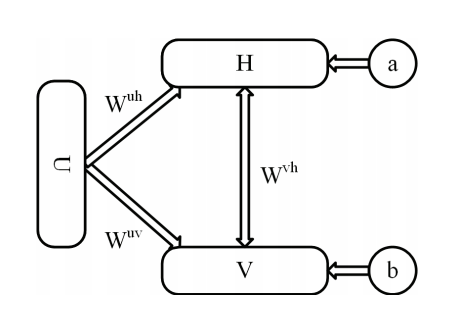
\includegraphics[width=0.8\columnwidth, height=7cm]{images/crbm.png}
\par\end{centering}
\caption{\protect How CRBM works \cite{short-termElectricalLoad} \label{fig:crbm}}
\end{figure}

One study tried to apply and test the performance conditional restricted Boltzmann machine (CRBM) for forecasting short term demand of energy.  Institutional block (a university) and a guest house was used in collecting datasets for the study and discover that CRBM is better for an hour-ahead forecasting compared to day-ahead forecasting \cite{short-termElectricalLoad}.

It is plausible that the study focuses on short-term demand since it aims to observe the consumption of the electricity and in the end, efficiently manage it.

\subsection{Extended Nearest Neighbor (ENN)}

Extended Nearest Neighbor (ENN) is a newly developed algorithm where it based its classification on the maximum gain of intra-class coherence \cite{ElectricityLoadProfileData-ENN}.  It uses generalized classwise statistics in order to obtain intraclass coherence.  A general formula for ENN is shown below,

\begin{equation} \label{ENN}
f_{ENN}=arg\max \Theta ^{j}\\j\in 1,2,\ldots 
= arg\max \sum _{i=1}^{i}T_{i}^{j}\\j\in 1,2,\ldots
\end{equation}

where $f_{ENN}$ is the ENN classifier $\Theta ^{j}$ is the intraclass coherence, and $T_{i}^{j}$ be the generalized class-wise statistics.

One study used this in classifying electricity load profile of the customers by first predicting the load demand variability of the specified customers then predict the load demand of the customer.  The results showed that compared to traditional load profile classifications that focuses on the shape of the load profile or reducing the dimension of the created model, this approach focuses on getting its data and classify things directly from a smart metered gadget which makes the classification faster \cite{ElectricityLoadProfileData-ENN}.


\section{Summary}
Researches in energy management are becoming popular and lots of techniques are already discovered and being used in other parts of the world.  Unfortunately, there is not much in the country since datasets of load profiles of the appliances used are not available. However, the techniques being used for energy utilization can be applied in the context of our country. In the end, we decided to use ELM for PV power forecasting due its advantages with accuracy and learning speed over the other techniques. We also decided to use ENN for load forecasting since it has shown to have high accuracy and can classify things directly from a smart metered gadget.

\begin{table}[H]
\caption{Summary of PV Power Forecasting Techniques}
\centering
\begin{tabular}{|c|c|c|}
\hline
\textbf{Model} & \textbf{Accuracy} & \textbf{Learning Speed} \\ \hline
ARIMA          & Low               &                         \\ \hline
kNN            & Low               &                         \\ \hline
ANN            & High              & Slow                    \\ \hline
ELM            & High              & Fast                    \\ \hline
\end{tabular}
\end{table}

\begin{table}[H]
\caption{Summary of Load Forecasting Techniques}
\centering
\begin{tabular}{|c|c|c|}
\hline
\textbf{Model} & \textbf{Pros}          & \textbf{Cons}               \\ \hline
FFT            & Efficient, Linear      & Low Accuracy                \\ \hline
GRG            & More accurate than FFT & Gradient Method Limitations \\ \hline
CRBM           & High Accuracy          & Dataset Dependent           \\ \hline
ENN            & High Accuracy          & Dataset Dependent           \\ \hline
\end{tabular}
\end{table}

\cleardoublepage{}

\chapter{Problem Statement and Objectives \label{cha:ProbStatement}}

\section{Problem Statement}

%%condense, solution directly address the need
%% walang dataset, in other parts of the country, pawala wala kuryente

%% wala pa ung need at ung solution tsaka benefits

% needs 1-2 sentences - walang system para mamaximize ng solar energy sa bansa since wala pa ring dataset available na applicable sa Pinas

% differentiation - what's already there but not enough
% maraming datasets available out there kaso hindi pwedeng gamitin sa PH setting dahil sa maraming factors

% solution - creation ng dataset applicable for PH setting -> creation ng hybrid solar-grid system with its own energy management system for the common household

% benefits - maximize the use of available energy resources and less expensive compared to a fully solar system

Solar energy is an emerging power source in the country since it is renewable, however, as of now, the country cannot maximize this kind of power source.  Implementing a purely solar dependent power source is expensive and impractical.  One possible solution is the application of a hybrid solar-grid system with its own energy management system wherein it can predict the state of charge, incoming PV power, and load demand of the consumer.  To achieve accurate prediction, a proper dataset for analysis is needed.  Thus, there is a need for a dataset that describes the load profiles of appliances applicable in the Philippine setting and an energy management system for maximizing the usage of solar energy.

\section{Objectives}
The project aims to create a system that will automatically determine whether to use solar power or an electric grid to power a specific appliance based on weather and load profile of the household and a web application to view the load profile of each appliance.  In order to make the system appropriate in the Philippine household context, information on load profiles of commonly used appliances in the country has to be obtained.  The target system is composed of the following:

\begin{itemize}
    \item A main controller that will automatically determine whether to use a smart grid or a battery to power a specific appliance based on weather and load profile of the household
    \item a web application to view the load profile of each appliance and a smart plug that will monitor the energy consumption of each appliances
    \item dataset of load profiles of commonly used appliances in the country
\end{itemize}

\section{Scope and Limitations}
%% The system will forecast electric consumption hourly.
%% collect dataset at school grounds
%%summer
%%fields on dataset to methodology
First, the dataset to be created will only describe the behavior of appliances during summertime since it is the time of collection of data.  The data will be collected from a simulated household environment wherein this environment will represent how often Filipinos use each appliances to be examine in the project.

On the other hand, since a dataset is needed to create the controller for it to learn the behavior of the appliances, and no existing datasets are present that is applicable the the Philippines as of the moment, a synthetic dataset will be created.  This synthetic dataset will come from other existing datasets that were created with almost the same conditions as summertime in the country.

Lastly, the controller to be created in the study will only output the recommendation for which energy source is to be used in supplying the appliances and will not handle the actual switching of energy source.

% simulated household environment
% 220W

\cleardoublepage{}

\chapter{Methodology\label{cha:Methodology}}

%This section discusses the methods and techniques that will be used to implement the project. This includes not only the actual implementation, but also how tests are designed and their results obtained and analyzed. The methodology may, if applicable, contain the following subsections: design, implementation, and testing. Alternative ways of organizing this section (that is more suited to the type of project being proposed) may be used.

% comments from sir
% State yung field ng datasets na relevant, very clear sa audience
% Metrics to measure: anong statistical tests yung gagamitin
% Fabrication technique na gagamitin sa data, bakit
% Ilang data points yung kukunin para sa measurements kahit estimate (interval, bakit ganun katagal yung interval, duration ng isang measurement, daytime ba o night time, etc)

\section{Design}

%Information on how the design will be obtained shall be presented. It shall be indicated whether the tools, parts, and algorithms that will be used in the project will be created by the author or taken from a different source.

The project will be divided into two main parts: the creation of dataset and the creation of the controller.

For the creation of dataset, smart plugs will be connected to each device will be used for power monitoring of each appliances.  The metrics to be measured and collected will be the following:
\begin{itemize}
    \item current levels of each appliance
    \item voltage levels of each appliance
    \item energy consumption of each appliance
    \item Conditions of the surroundings of the household (temperature, weather)
\end{itemize}

After collecting the metrics given, it will be organized and saved into an excel file.  The fields of the dataset will be the following:

\begin{itemize}
    \item type of appliance
    \item mode of operation
    \item time of usage per day
    \item power consumption per hour
    \item temperature per day
\end{itemize}

%For the creation of controller, a machine learning algorithm will be used for the controller to learn the behavior of the load profiles of the appliances used and be able to predict the amount of energy sources needed to supply the appliances used.  The inputs of the algorithm will be the same as the fields of the dataset to be created.

For the creation of controller, a machine learning algorithm will be used in the server to learn the behavior of the load profiles of the appliances used and be able to predict the amount of energy sources needed to supply the appliances used which will be used to decide the signals to be sent to the microcontroller.  For the inputs for the algorithm for PV forecasting, the data will be collected from Weather Underground, a commercial service that provides weather information over the internet, which has the factors needed for the model. The inputs of the algorithm for load forecasting will be the same as the fields of the dataset to be created, in addition to the actual consumption data that will be recorded.

The whole system to be implemented will consist of the following: energy supplies (one from solar power and one from an electric grid), a controller, the appliances to be used, and a web application for load monitoring of the appliances. Figure \ref{fig:sys-diag} shows an overview of the system.

\begin{figure}[H]
\begin{centering}
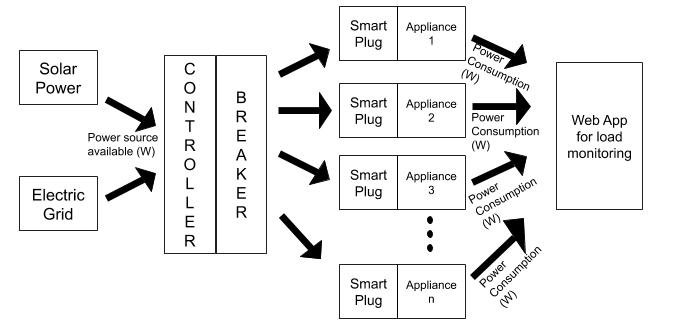
\includegraphics[width=0.8\columnwidth]{images/system_diagram.png}
\par\end{centering}
\caption{\protect System Overview \label{fig:sys-diag}}
\end{figure}

The setup of the controller is shown in Figure \ref{fig:control}.  The controller will be composed of the following: a server and a microcontroller.  The microcontroller will be the one to send and receive data needed for the decision making (whether to use solar power or electric grid as energy source). An Arduino Uno R3 board with an ATMega328 microcontroller will be used, due to its availability, price, has the ability to interact with the internet that is useful for sending the information to the server, and has I/O lines for detecting and sending inputs and outputs of the system respectively. On the other hand, the server will be the one to process the data from the microcontroller.  It will be the one to learn the behavior of the appliances using a machine learning algorithm and will be the one to decide whether to get energy source from the solar power or the electric grid.  The inputs of the controller are the current state of charge of the battery used for storing of the solar power, and the overall power consumption of the household.  The output will be the choice of energy source to be used in supplying the appliances.

\begin{figure}[H]
\begin{centering}
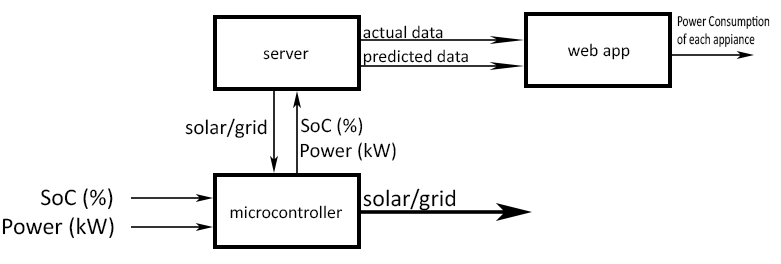
\includegraphics[width=0.8\columnwidth]{images/control.png}
\par\end{centering}
\caption{\protect Controller of the system \label{fig:control}}
\end{figure}

On the other hand, the web application for viewing the power consumption of the appliances will be done through HTML, CSS and JavaScript.  The user of the application will be able to view the power consumption of the appliances either hourly, daily, weekly, or monthly.  They can also have the choice whether to view the consumption through tables, or through graphs so that they can easily view the trend of their consumption.  The application will only be limited to one user.  Figure \ref{fig:web-app} shows a sample layout of the web application.

\begin{figure}[H]
\begin{centering}
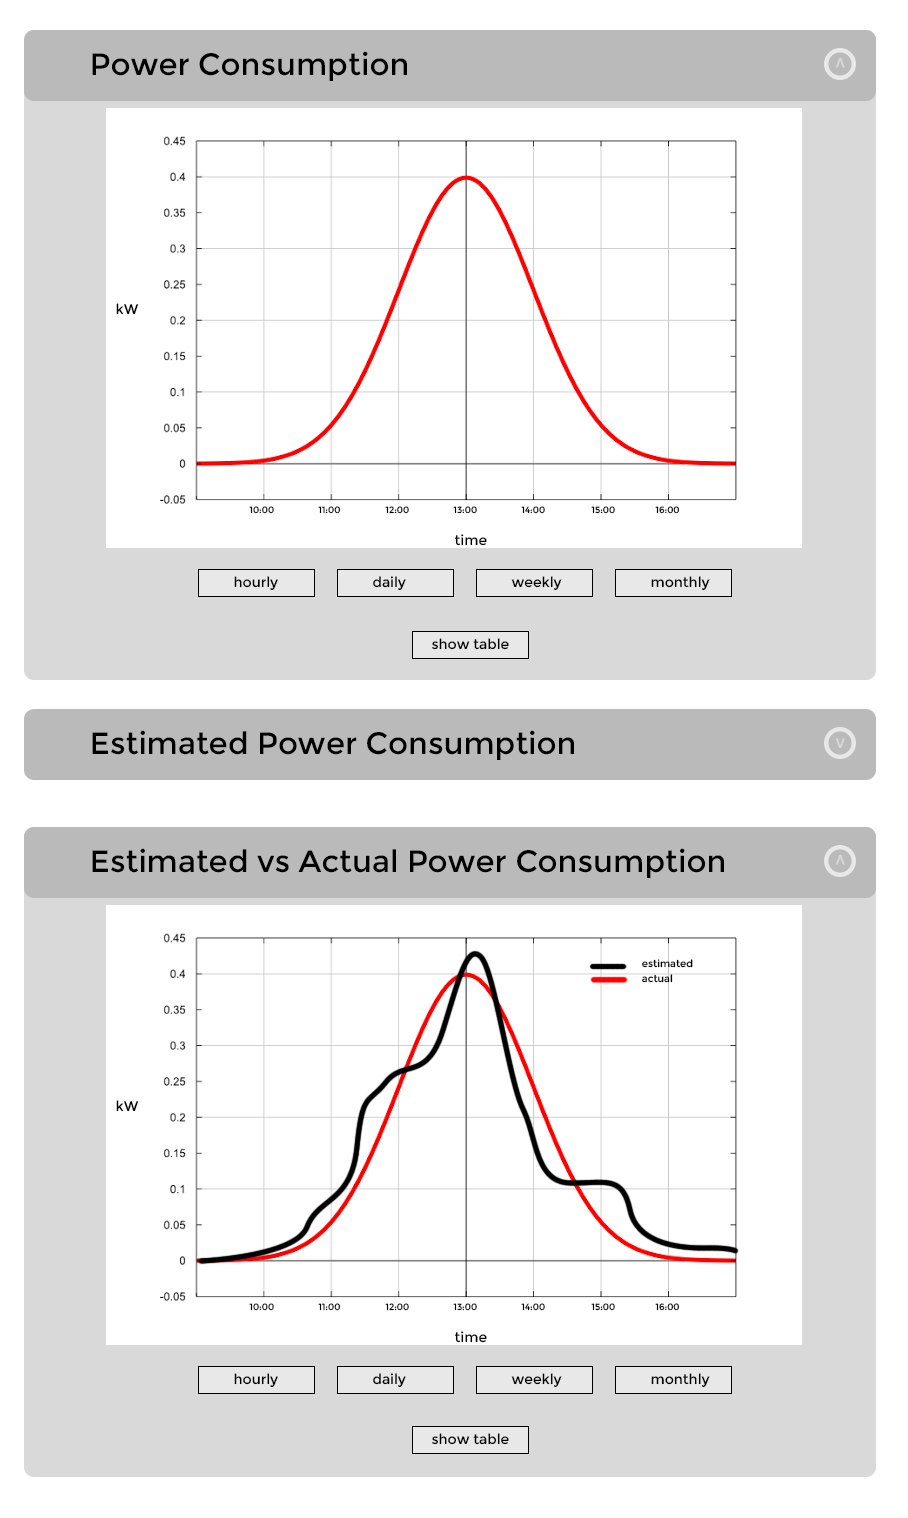
\includegraphics[height=4in]{images/web-app.png}
\par\end{centering}
\caption{\protect Sample Layout of the Web Application \label{fig:web-app}}
\end{figure}

For the smart plugs, it will be divided into three modules, the relay board that can handle 220V AC input from the outlet, the microcontroller with RF module, and the CS5464.  It will be design using a modular approach like in Smart Domotix \cite{Domotix} to decrease the size of the smart plug and to isolate RF module and CS5464 that can only handle 5V DC input to 220V from the microcontroller.  Circuit of the smartphone charger will be used for the conversion of 220V to 5V.  The schematic diagrams and board layouts of each of the smart plug is shown in Figures \ref{fig:main-board}, \ref{fig:atmega}, and \ref{fig:cs5464}.

%% main board
\begin{figure}[H]
    \centering
  \subfloat[Schematic Diagram\label{fig:main-board-schem}]{%
       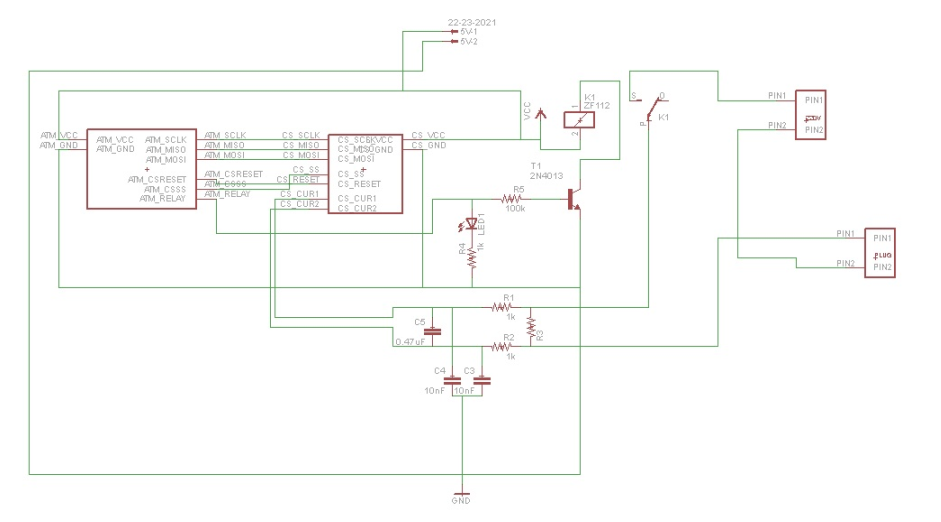
\includegraphics[width=\columnwidth]{images/main_board_schematic.png}}
    \hfill
    \\
  \subfloat[Board Layout\label{figmain-board-layout}]{%
        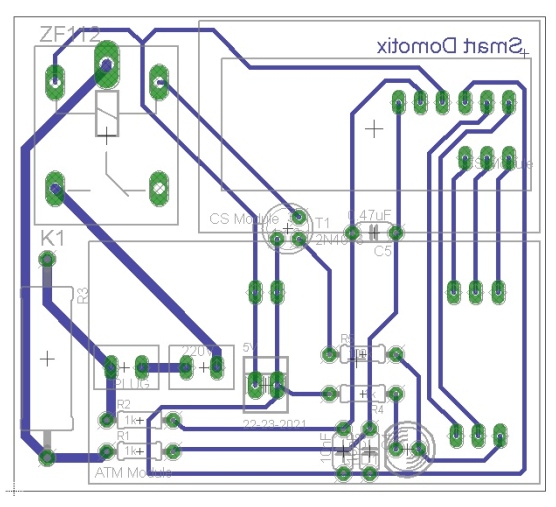
\includegraphics[width=0.2\linewidth]{images/main_board_layout.png}}
  \caption{ Main Board \cite{Domotix}} \label{fig:main-board}
\end{figure}

%%atmega
\begin{figure}[H]
    \centering
  \subfloat[Schematic Diagram\label{fig:atmega-schem}]{%
       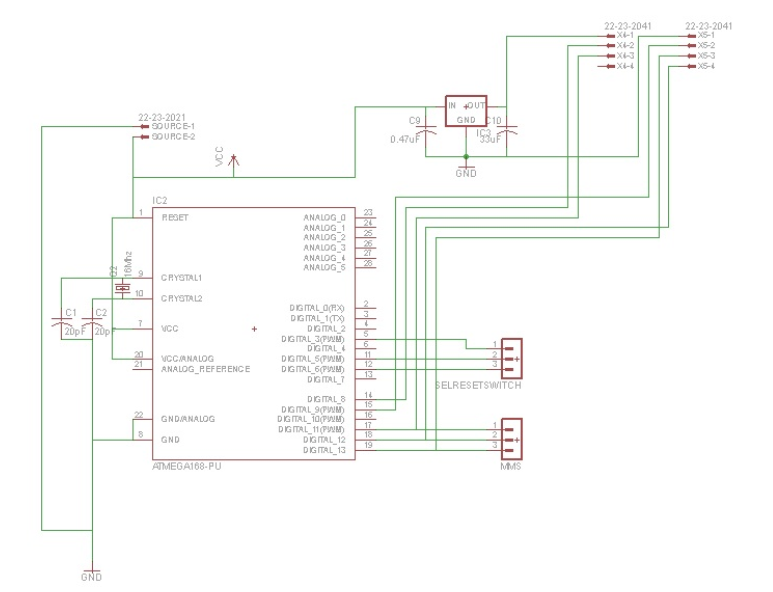
\includegraphics[width=\columnwidth]{images/atmega-schematic.png}}
    \hfill
    \\
  \subfloat[Board Layout\label{fig:atmega-layout}]{%
        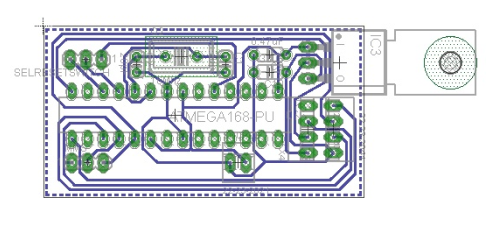
\includegraphics[width=0.5\linewidth]{images/atmega-layout.png}}
  \caption{ ATMega328 Microncontroller \cite{Domotix}} \label{fig:atmega}
\end{figure}

%%CS5464
\begin{figure}[H]
    \centering
  \subfloat[Schematic Diagram\label{fig:cs5464-schem}]{%
       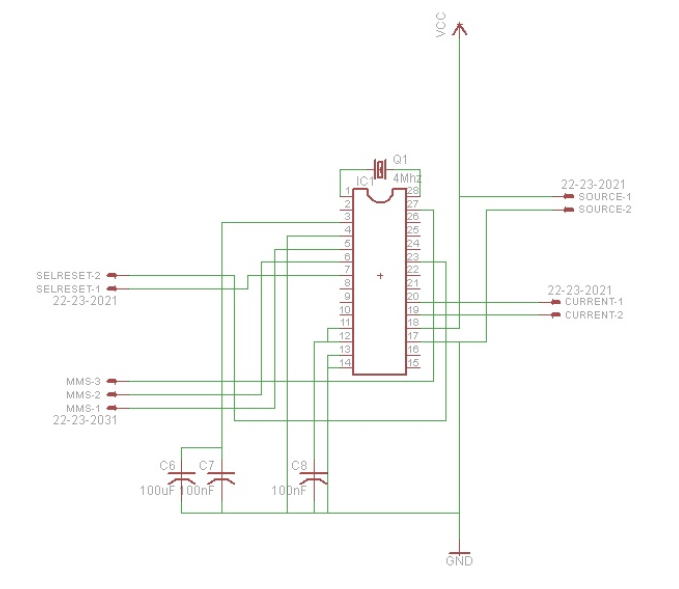
\includegraphics[width=\columnwidth]{images/cs5464-schematic.png}}
    \hfill
    \\
  \subfloat[Board Layout\label{fig:cs5464-layout}]{%
        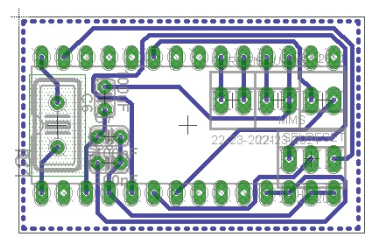
\includegraphics[width=0.4\linewidth]{images/cs5464-layout.png}}
  \caption{ CS5464 Module \cite{Domotix}} \label{fig:cs5464}
\end{figure}

\section{Implementation}

%Information on how the design will be implemented shall be presented. It shall be indicated if the labor is to be performed by the author or by a different source. 

For the creation of the dataset, a simulated household environment will be used for the collection of data. The appliances to be included will be based from a survey  conducted by the Philippine Statistics Authority and are as follows: compact fluorescent lamp, linear fluorescent lamp, television, radio, electric fan, air conditioning unit, flat iron, desktop computer, rice cooker, and portable water heater \cite{top}. The said set-up will be located in the Solar Laboratory, Electronics and Electrical Engineering Institute, University of the Philippines Diliman.

A survey will be conducted by the researchers around the community near University of the Philippines - Diliman. Consisting of 30 households, the questions of the survey will be the following:

\begin{itemize}
    \item how long do they use the specified appliances per day
    \item Mode of Operation they use in each appliances
    \item time of usage per day for each appliances
\end{itemize}

Software based from Python will be used to collect data from smart plugs and all metrics will be measured per day with a time interval of one minute.  The measured data will have four decimal places. All data will then be saved to a centralized database which will contain all of the measured data.  The collection will be done for five weeks.

Software based from Python will also be used for the creation of controller since Python already has modules that can make the implementation of the machine learning algorithm faster and easier.

After integrating all parts of the system, the system will then be implemented and will be monitored hourly if it can provide the energy needs of each appliances.

%algo to be used

\section{Testing}
%Information on how the design and the implementation will be tested shall be presented. Moreover, information on how the test results will be evaluated against the specifications or goals of the project shall also be stated.

Upon creation and processing of the dataset, the metric to be considered for testing it is its usability and reliability.  It will be tested using disaggregation algorithms readily available online..

For the controller, the metric to be considered for testing is the accuracy of the predicted values of the controller for the state of charge of the battery, and the energy needed to supply the appliances.  For the accuracy, the predicted values will be compared with the actual values of the state of charge, and the actual power needed by the appliances. This will then be evaluated by calculating its root mean square error (RMSE) in order to verify the results.

\begin{equation} \label{eq:RMSE}
    RMSE = \sqrt{\frac{\sum\limits_{i=1}^{N} \left(X_1 - X_2 \right)^2}{N}}
\end{equation}


\cleardoublepage{}

%\chapter{Preliminary Findings\label{cha:Prelims}}

%%test algo , libraries, etc
% This is an optional chapter where you present all of your preliminary
% work, results, and analysis. For final project documentations, this
% chapter becomes the Results and Analysis chapter.

%\cleardoublepage{}

\chapter{Project Schedule and Deliverables\label{cha:Project-Sked}}
%For final project documentations, this chapter becomes the Conclusions and Recommendations chapter.

%For project proposals, end the documentation by presenting the project schedule and expected deliverables. This section should clearly describe the activities that will be done. Important milestones should be indicated in the schedule of activities. It should be as specific as possible.

The project will be done in a period of 16 weeks.  The schedule of work will be seen below.

\section{Gantt Chart}

% This is a time table that clearly indicates the important milestones
% of the project. The schedule should be divided into weekly segments.
% The authors should make sure that the schedules are realistic. It
% is advised that the weekly tasks are as detailed as possible.

\begin{figure}[]
\begin{centering}
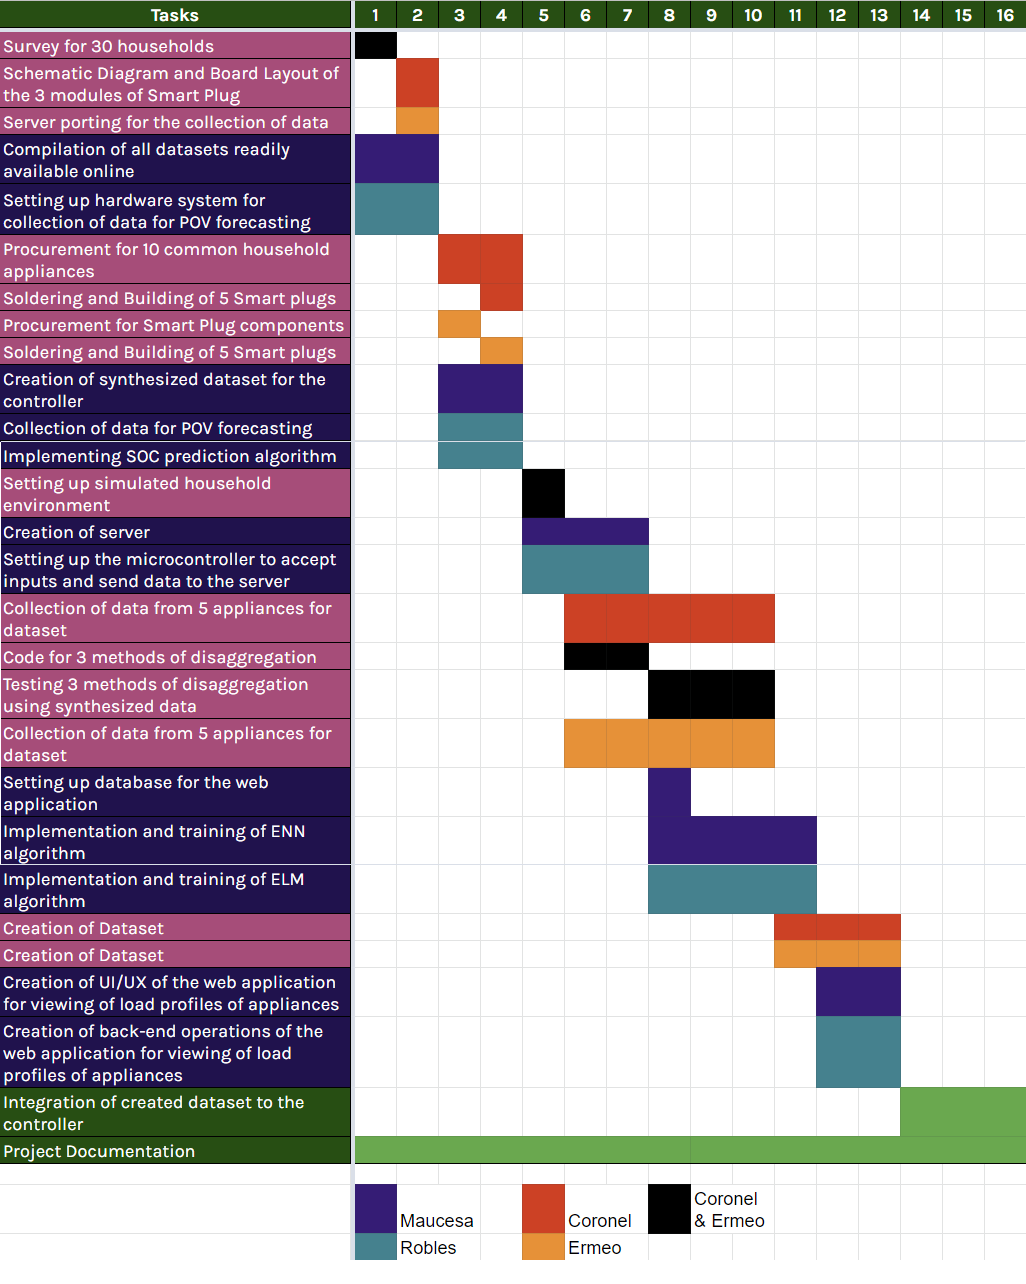
\includegraphics[ height=8in]{images/gantt_chart.png}
\par\end{centering}
\caption{\protect Gantt Chart for 16 Weeks \label{fig:gantt-chart}}
\end{figure}

Based on the gantt chart in Figure \ref{fig:gantt-chart}, the tasks in Violet will be done by Maucesa, the tasks in blue will be done by Robles, the tasks in orange will be done by Ermeo, the tasks in red will be done by Coronel, and the tasks in black will be done by Ermeo and Coronel.  Lastly, the tasks in green will be done by everyone.

\section{Project Deliverables}

% This section should clearly point out and describe the expected outputs
% at halfway-point. If the project will be done by a group, the deliverables
% of each group member shall be clearly and specifically stated. 
For the halfway-point deliverable, Coronel and Ermeo should be done with the surveying, simulated household environment, and half of the data collection for the dataset. Alongside this, Maucesa and Robles should be done with the creation of the synthesized dataset for the controller, and creation of the controller for the system should be initiated.

The final deliverable will be the created dataset of load profiles, the creation of controller is already done and integrated to the dataset created and the web application for viewing the load profiles of the appliances.

\cleardoublepage{}

\bibliographystyle{unsrt}
\nocite{*}
\bibliography{bibliography}

\cleardoublepage{}

\end{document}
